\documentclass[mathserif,compress]{beamer}

\mode<presentation>
{
  \usecolortheme{}
  \definecolor{blue}{rgb}{0.8,0,0}
\setbeamercolor{ separation line }{bg=black}
  \setbeamercolor{frametitle}{bg=gray!20!white}
  \setbeamertemplate{footline}{% 
  \hfill% 
  \usebeamercolor[fg]{page number in head/foot}% 
  \usebeamerfont{page number in head/foot}% 
  \insertframenumber%
  %\,/\,\inserttotalframenumber
  \kern1em\vskip2pt% 
}
}

\makeatletter
\def\mytitleframe{\bgroup
\setbeamertemplate{footline}
{
  \leavevmode%
  \hbox{%
  \begin{beamercolorbox}[wd=.333333\paperwidth,ht=2.25ex,dp=1ex,center]{author in head/foot}%
    \usebeamerfont{author in head/foot}\insertshortauthor\expandafter\beamer@ifempty\expandafter{\beamer@shortinstitute}{}{~~(\insertshortinstitute)}
  \end{beamercolorbox}%
  \begin{beamercolorbox}[wd=.333333\paperwidth,ht=2.25ex,dp=1ex,center]{title in head/foot}%
    \usebeamerfont{title in head/foot}\insertshorttitle
  \end{beamercolorbox}%
  \begin{beamercolorbox}[wd=.333333\paperwidth,ht=2.25ex,dp=1ex,right]{date in head/foot}%
    \usebeamerfont{date in head/foot}\insertshortdate{}\hspace*{2em}
%    \insertframenumber{} / \inserttotalframenumber\hspace*{2ex} 
    \hspace*{6ex}
  \end{beamercolorbox}}%
  \vskip0pt%
}
\maketitle
\egroup
\addtocounter{framenumber}{-1}
}
\makeatother

\newcommand\hmmax{0}
\newcommand\bmmax{0}
\usepackage{natbib, verbatim}

\usepackage[utf8]{inputenc}

\usepackage{mathpazo}
\usepackage[T1]{fontenc}

\usepackage{amsmath}
\usepackage{amsthm}
\usepackage{amssymb}
\usepackage{mathptmx}
\usepackage{anyfontsize}
\usepackage{t1enc}
\usepackage{appendix}
\usepackage{array}
\usepackage{bm}
\usepackage{cancel}
\usepackage[font=small,labelfont=bf]{caption}
\usepackage{cite}
\usepackage{courier}
\usepackage{graphicx}
\usepackage{empheq}
\usepackage{enumerate}
\usepackage{listings}
\usepackage{mathtools}
\usepackage{units}
\usepackage{bigstrut}
\usepackage{rotating}
\usepackage{ mathrsfs }
\usepackage{multirow}
\usepackage{booktabs}
\usepackage{algorithm, algorithmic}

\DeclareMathAlphabet{\mathcal}{OMS}{cmsy}{m}{n}

\DeclareMathAlphabet{\mathsfit}{\encodingdefault}{\sfdefault}{m}{}
\SetMathAlphabet{\mathsfit}{bold}{\encodingdefault}{\sfdefault}{bx}{}

\newcommand{\tens}[1]{\bm{\mathsfit{#1}}}

\usepackage{color}
\lstset{language=R,basicstyle=\ttfamily,breaklines=true,
                keywordstyle=\color{blue}\ttfamily,
                stringstyle=\color{red}\ttfamily,
                commentstyle=\color{magenta}\ttfamily,
                showstringspaces=false,
                }

\newcommand*\widefbox[1]{\fbox{\hspace{2em}#1\hspace{2em}}}
\newcommand*\mb{\mathbf}
\newcommand*\reals{\mathbb{R}}
\newcommand*\complex{\mathbb{C}}
\newcommand*\naturals{\mathbb{N}}
\newcommand*\nats{\naturals}
\newcommand*\integers{\mathbb{Z}}
\newcommand*\rationals{\mathbb{Q}}
\newcommand*\irrationals{\mathbb{J}}
\newcommand*\pd{\partial}
\newcommand*\htab{\hspace{4 mm}}
\newcommand*\vtab{\vspace{0.5 in}}
\newcommand*\lsent{\mathcal{L}}
\newcommand*\conj{\overline}
\newcommand*\union{\cup}
\newcommand*\intersect{\cap}
\newcommand*\cl{\cancel}
\newcommand*\ANS{\text{ANS}}
\newcommand*\As{\text{As}}
\newcommand*\then{\rightarrow}
\newcommand*\elim{\text{E}}
\newcommand*\intro{\text{I}}
\newcommand*\absurd{\curlywedge}
\newcommand*\NK{\vdash_{\text{NK}}}
\newcommand*\derivation{\begin{tabular} { >{$}l<{$}  >{$}c<{$}  >{$}l<{$}  >{$}r<{$} }}
\newcommand*\interp{\mathcal{I}}
\newcommand*\ba{\[ \begin{aligned}}
\newcommand*\ea{\end{aligned} \]}
\newcommand*\C{\mathcal{C}}
\newcommand*\D{\mathscr{D}}
\newcommand*\e{\operatorname{e}}
\newcommand*\df{=_{\text{def}}}
\newcommand*\eps{\epsilon}
\newcommand*\enum{\begin{enumerate}[label=(\alph*)]}
\newcommand*\enumend{\end{enumerate}}
\newcommand*\E[1]{\tens{E}\left[#1\right]}
\newcommand*\Esub[2]{\tens{E}_{#1}\left[#2\right]}
\newcommand*\Var[1]{\tens{Var}\left[#1\right]}
\newcommand*\Cov[1]{\tens{Cov}\left[#1\right]}
\newcommand*\iid{\overset{\text{iid}}{\sim}}
\newcommand*\Exp[1][\lambda]{\text{Exp}(\text{rate}=#1)}
\newcommand*\ind[1]{\mathbb{1}\left(#1\right)}
\newcommand*\set[1]{\left\{#1\right\}}
\newcommand*\estim[1]{\widehat{#1}}
\newcommand*\der{\text{d}}
\newcommand*\norm[1]{\left\|#1\right\|}
\newcommand*\dist[2]{\;\text{dist}\left(#1, #2\right)}
\newcommand*\interior{\text{int}\;}
\newcommand*\exterior{\text{ext}\;}
\newcommand*\boundary{\text{bd}\;}
\newcommand*\lh{\overset{\text{L'H}}{=}}

\renewcommand\Re{\operatorname{Re}}
\renewcommand\Im{\operatorname{Im}}
\DeclareMathOperator*{\argmin}{arg\;min}
\DeclareMathOperator*{\argmax}{arg\;max}
\renewcommand\;{\,}
\renewcommand\epsilon{\varepsilon}
\renewcommand\rho{\varrho}
\renewcommand\phi{\varphi}
\renewcommand\mod{\hspace{0.2em} \textbf{mod}\hspace{0.2em}}
\renewcommand\Pr[1]{ \mathsf{Pr}\left(#1\right) }
\def\ci{\perp\!\!\!\perp}

\usepackage{tikz}
\usetikzlibrary{positioning}
\usetikzlibrary{shapes,arrows}
\usepackage{adjustbox}

\tikzstyle{decision} = [diamond, draw, fill=blue!20, 
    text width=4.5em, text badly centered, node distance=3cm, inner sep=0pt]
\tikzstyle{block} = [rectangle, draw, fill=blue!20, 
    text width=6em, text centered, rounded corners, minimum height=4em]
\tikzstyle{line} = [draw, -latex']
\tikzstyle{cloud} = [draw, ellipse,fill=red!20, node distance=3cm,
    minimum height=2em]

\lstset{breaklines=true,
        numbersep=5pt,
        xleftmargin=.25in,
        xrightmargin=.25in}

\DeclareMathOperator{\sech}{sech}
\DeclareMathOperator{\sgn}{sgn}
\makeatletter
\renewcommand*\env@matrix[1][*\c@MaxMatrixCols c]{%
  \hskip -\arraycolsep
  \let\@ifnextchar\new@ifnextchar
  \array{#1}}
\makeatother

\newenvironment{amatrix}[1]{%
  \left(\begin{array}{@{}*{#1}{c}|c@{}}
}{%
  \end{array}\right)
}

\lstset{basicstyle=\footnotesize\ttfamily,breaklines=true}


\newcommand{\real}{\ensuremath{\mathbb{R}}}
\newcommand{\bA}{\mbox{\protect\boldmath $A$}}
\newcommand{\bo}{\mbox{\protect\boldmath $o$}}
\newcommand{\bu}{\mbox{\protect\boldmath $u$}}
\newcommand{\by}{\mbox{\protect\boldmath $y$}}
\newcommand{\bx}{\mathbf{x}}
\newcommand{\bs}{\mbox{\protect\boldmath $s$}}
\newcommand{\bS}{\mbox{\protect\boldmath $S$}}
\newcommand{\bz}{\mathbf{z}}
\newcommand{\bh}{\mbox{\protect\boldmath $h$}}
\newcommand{\bF}{\mbox{\protect\boldmath $f$}}
\newcommand{\bt}{\mbox{\protect\boldmath $t$}}
\newcommand{\bc}{\mbox{\protect\boldmath $c$}}
\newcommand{\bC}{\mbox{\protect\boldmath $C$}}
\newcommand{\bp}{\mathbf{p}}
\newcommand{\bV}{\mbox{\protect\boldmath $V$}}
\newcommand{\bX}{\mbox{\protect\boldmath $X$}}
\newcommand{\bW}{\mbox{\protect\boldmath $W$}}
\newcommand{\bZ}{\mbox{\protect\boldmath $Z$}}
\newcommand{\bof}{\mbox{\protect\boldmath $f$}}
\newcommand{\indicator}{{\ensuremath{\mathbb{I}}}}
\newcommand{\M}{{\ensuremath{\rm M}}}
\newcommand{\bbeta}{\boldsymbol{\beta}}
\newcommand{\balpha}{\boldsymbol{\alpha}}
\newcommand{\bgamma}{\boldsymbol{\gamma}}
\newcommand{\bdelta}{\boldsymbol{\delta}}
\newcommand{\bmu}{\boldsymbol{\mu}}
\newcommand{\bSigma}{\boldsymbol{\Sigma}}
\newcommand{\btheta}{\protect\boldsymbol{\theta}}
\newcommand{\bzero}{\mathbf{0}}
\newcommand{\hsp}{\hspace{0.2mm}}

\footnotesize

\beamertemplatenavigationsymbolsempty
\setbeamertemplate{headline}{\vskip2pt}

\title[]{Combining Mixture Components for Clustering}

\author[]
{Jean-Patrick Baudry, Adrian E. Raftery, Gilles Celeux, Kenneth Lo, and Rapha$\ddot{\text e}$l Gottardo\\$\;$ \\Presented by Branden Olson}

\date[]
{June 13, 2018}

\institute[]
{
}

%Prepare a short presentation based on your chosen paper (10 slides at most). The main points you need to cover are:
%
%1. What is the scientific problem your paper is considering?
%
%2. What has been done to solve this problem before (aka literature review)?
%
%3. What new ideas do the authors propose?
%
%4. What are the interesting findings of the experiments on real data?
\AtBeginSection[]
{
   \begin{frame}
       \frametitle{Outline}
       \tableofcontents[currentsection]
   \end{frame}
}

\begin{document}

\mytitleframe

\section{Introduction} 

\begin{frame}\frametitle{Scientific Problem}
\begin{itemize}
\item[]
\alert{Goal:} cluster data into groups
\bigskip
\item[]
\alert{Def'n. of groups}: "Contiguous, densely-populated regions of feature space, separated by contiguous, relatively empty regions"
\bigskip
\item[]
\alert{Difficulty:} \# of groups often unknown
\end{itemize}
\end{frame}

\begin{frame}\frametitle{Example clustering of data in $\reals^2$}
\begin{center}
\begin{minipage}{0.45\linewidth}
\includegraphics[width=\linewidth]{unclustered.pdf}
\begin{center}
Unclustered
\end{center}
\end{minipage}
\hfill
\begin{minipage}{0.45\linewidth}
\includegraphics[width=\linewidth]{clustered.pdf}
\begin{center}
Clustered \& labeled
\end{center}
\end{minipage}
\end{center}
\end{frame}

\begin{frame}\frametitle{Model-based clustering}
\begin{itemize}
\item[]
\alert{Our focus:} model-based clustering
\bigskip
\item[]
\alert{Assumption:} each data point $\bx_i \sim$ \emph{Gaussian mixture density} with $K$ components:

\ba
f(\bx_i ; K, \theta_K) 
	& = \sum_{k=1}^K p_k
		\phi \left(\bx_i ; \mu_k, \Sigma_k\right),
		\htab
		1 \le i \le n
\ea
\begin{itemize}
\item
$\bp = (p_1, \dotsc, p_K)$: mixture proportions
\bigskip
\item
$\pmb\mu = (\mu_1, \dotsc, \mu_K)$: component means
\bigskip
\item
$\pmb\Sigma = (\Sigma_1, \dotsc, \Sigma_K)$: component covariances
\bigskip
\item 
$\theta_K = (\bp, \bmu, \pmb\Sigma)$: total parameter vector
\end{itemize} 
\end{itemize}
\end{frame}

\begin{frame}\frametitle{Model-based clustering}
\begin{itemize}
\item[] \alert{Caveat:} Each group corresponds to a mixture component
\bigskip
\item[]
\alert{Pro:} Can estimate \# of components \& parameters easily
\bigskip
\begin{itemize}
\item E.g. Expectation-Maximization (EM) algorithm
\end{itemize}
\bigskip
\item[]
\alert{Cons:} What if the groups are non-Gaussian?
\end{itemize}
\end{frame}

\begin{frame}\frametitle{Model selection}
\begin{itemize}
\item[]
Start with set of candidates $\set{K_\text{min}, \dotsc, K_\text{max}}$ 
\bigskip
\item[]
For each $K$ in the set, 
compute the MLE 
$\estim\theta_K = (\estim{\mathbf p}, \estim{\pmb\mu}, \estim{\pmb\Sigma})$
\bigskip
\item[]
\alert{Goal}: Choose the ``best'' model $\left(\estim K, \estim\theta_{\estim K}\right)$, according to some criterion
\end{itemize}
\end{frame}

\section{Previous work: BIC}
\begin{frame}\frametitle{Bayesian Information Criterion (BIC)}
\begin{itemize}
\item[]
Dasgupta \& Raftery (1998): $\estim K = \argmax_K \text{BIC}(K)$, where
\ba
\text{BIC}(K)
	= \underbrace{\log \; f(\bx; K, \estim\theta_K)}_\text{\alert{observed} log-likelihood} 
	- \underbrace{\frac{\nu_K \log(n)}{2}}_\text{penalty}
\ea
\begin{itemize}
\item
$f(\bx; K, \estim\theta_K) = \prod_{i=1}^n f(\bx_i; K, \estim\theta_K)$
\bigskip
\item
$\estim\theta_K = $ MLE for parameters
\bigskip
\item
$\nu_K = \# $ of free parameters in $K$-component model
\end{itemize}
\end{itemize}
\end{frame}

\begin{frame}\frametitle{BIC: Remarks}
\begin{itemize}
\item[]
\alert{Pro:} Estimates \# of components well insofar as the Gaussian approximation holds
\bigskip
\item[]
\alert{Con:} Infers non-Gaussian groups as a combination of multiple Gaussian components
\begin{itemize}
\bigskip
\item
Overestimates the \# of groups, since each component represents a group
\end{itemize}
\end{itemize}

\end{frame}

\begin{frame}\frametitle{Problematic example}
\begin{itemize}
\item[]
Simulate 500 points from unit square in $\reals^2$ \& 200 points from a 
$\mathcal N_2\left(\begin{pmatrix} 1 \\ 2 \end{pmatrix},
	\begin{pmatrix} 1/5 & 0 \\ 0 & 1/5 \end{pmatrix}\right)$:
\begin{center}
\includegraphics[width=0.5\linewidth]{../Olson/Figures/unif/unclustered.pdf}
\end{center}
\item[]
Assume spherical covariances, get $\estim\theta_K$  for each $K \in \set{1, \dotsc, 10}$, \& compute $\estim K_\text{BIC}$
\end{itemize}
\end{frame}

\begin{frame}\frametitle{Illustration: $K = \estim K_\text{BIC} = 5$}
Clustered, labelled data \& contours of estimated densities:
\begin{center}
\includegraphics[width=0.55\linewidth]{../Olson/Figures/unif/merged_5_contour.pdf}
\end{center}
\begin{itemize}
\item
BIC yields 5 components/clusters, but there are only 2 groups
\end{itemize}
\end{frame}

\section{Previous work: ICL}
\begin{frame}\frametitle{Completed likelihood}
\begin{itemize}
\item[]
Biernacki et al. (2000): consider the \text{\color<1>[rgb]{0,0.7,0}{completed}} likelihood
\ba
f(\bx_i, \text{\color<1>[rgb]{0,0.7,0}{$\bz_i$}} ; K, \estim\theta_K)
	& = \sum_{k=1}^K p_k \phi(\bx_i; \mu_k, \Sigma_k) 
		\text{\color<1>[rgb]{0,0.7,0}{$z_{ik}$}},
		\htab
		1 \le i \le n
\ea
\begin{itemize}

\item
$z_{ik} = \ind{ \bx_i \text{ arises from component } k}$
\bigskip
\item 
$\bz_i = (z_{i1}, \dotsc, z_{iK})$: standard basis vector in $\reals^K$
\bigskip
\item
$\bz = (\bz_1, \dotsc, \bz_n)$: $K \times n$ binary matrix
\end{itemize}
\bigskip
\item[]
The $\bz_i$ are unobserved, but we can estimate them!
\end{itemize}
\end{frame}

\begin{frame}\frametitle{Integrated Completed Likelihood (ICL) criterion}
\begin{itemize}
\item[]
So, instead choose $\estim K = \argmax_K \text{ICL}(K)$, where
\ba
\text{ICL}(K)
	= \underbrace{\log \; f(\bx, \text{\color<1>[rgb]{0,0.7,0}{$\estim\bz$}}; K, \estim\theta_K)}_\text{\alert{"completed"} log-likelihood} - \frac{\nu_K \log(n)}{2}
\ea
\begin{itemize}
\item
$f(\bx, \estim\bz) = \prod_{i=1}^n f(\bx_i, \estim\bz_i; K, \estim\theta_K)$
\bigskip
\item
$\estim\bz_i$ = the most likely cluster assignment of $\bx_i$ given $\estim\theta_K$
\end{itemize}
\end{itemize}
\end{frame}

\begin{frame}\frametitle{ICL: Under the hood}
\begin{itemize}
\bigskip
\item[]
Can show ICL penalizes entropy of clustering:

\ba
\text{Entropy}(K) = - \sum_{i=1}^n \sum_{k=1}^K
	t_{ik}(\estim\theta_K) \log t_{ik}(\estim\theta_K)
\ea
where
\ba
t_{ik}(\estim\theta_K) & = \Pr{\bx_i \text{ arises from component $k$} \;\bigg|\; \estim\theta_K } \\
	& = \frac{ p_k \phi_k(\bx_i | \mu_k, \Sigma_k)  }
 	{ \sum_{j=1}^K p_j \phi_j(\bx_i | \mu_j, \Sigma_j) }
\ea
\end{itemize}
\end{frame}

\begin{frame}\frametitle{ICL: Remarks}
\begin{itemize}
\item[]
\alert{Pro:} Better estimates \# of \emph{groups}, even under model misspecification
\bigskip
\item[]
\alert{Con:} Can underestimate \# of \emph{components}
\begin{itemize}
\bigskip
\item
Often includes poorly separated groups into one cluster 
\end{itemize}
\bigskip
\item[]
\alert{Question:} Does each component really represent a separate cluster? 
\end{itemize}
\end{frame}

\section{New contributions}
\begin{frame}\frametitle{Methodology}
\begin{itemize}
\item[]
\alert{Baudry et al.:}
Let's exploit respective strengths of BIC \& ICL!
\bigskip
\begin{enumerate}
\item
Start with BIC estimate of $K$ from initial set $\set{K_\text{min}, \dotsc, K_\text{max}}$
\bigskip
\item
At each stage, merge the 2 clusters which results in largest decrease in entropy
\bigskip
\item
Continue merging clusters, stopping at $K_\text{min}$
\end{enumerate} 
\bigskip
\item[]
Yields \emph{sequence of clusterings} for $K_\text{min}, \dotsc, \estim K_\text{BIC}$
\end{itemize}
\end{frame}

\begin{frame}\frametitle{Remarks}
\begin{itemize}
\item[]
Merging produces components that are \alert{Gaussian mixtures themselves}
\begin{itemize}
\bigskip
\item
Yields new conditional probabilities $t_{ik}$, influencing the entropy
\end{itemize}
\bigskip
\item[]
\alert{Key idea:} allows (\# components) $\ne$ (\# clusters)
\bigskip
\item[]
Complexity: $\mathcal O \left( \left\{\text{rate for } \estim K_\text{BIC} \right\}+ n K_\text{max}^3 \right)$
\end{itemize}
\end{frame}

\begin{frame}\frametitle{How to choose $K$}
\begin{itemize}
\item[]
Given our sequence of clusterings, how to choose $K$?
\bigskip
\item[]
Baudry et al. give a few suggestions:
\begin{enumerate}
\bigskip
\item
Subjectively, based on scientific background or examining plots
\bigskip
\item
Choosing $K = \estim K_\text{ICL}$
\bigskip
\item
Regressing entropy-based quantities on $K$ to identify a change point
\end{enumerate}
\bigskip
\item[]
Issues: Small-sample size, multiple change points (elbows)
\end{itemize}
\end{frame}

\begin{frame}\frametitle{Back to illustration}
\begin{itemize}
\item[]
Recall our simulation study and BIC solution:
\begin{minipage}{0.45\linewidth}
\includegraphics[width=\linewidth]{../Olson/Figures/unif/unclustered.pdf}
\begin{center}
Unclustered data
\end{center}
\end{minipage}
\hfill
\begin{minipage}{0.45\linewidth}
\includegraphics[width=\linewidth]{../Olson/Figures/unif/merged_5_contour.pdf}
\begin{center}
BIC solution ($K = 5$)
\end{center}
\end{minipage}
\end{itemize}
\end{frame}

\begin{frame}\frametitle{Merged solution, $K = \estim K_\text{BIC} = 5$}
\begin{center}
\includegraphics[width=0.7\linewidth]{../Olson/Figures/unif/merged_5_contour.pdf}
\end{center}
\end{frame}

\begin{frame}\frametitle{Merged solution, $K = 4$}
\begin{center}
\includegraphics[width=0.7\linewidth]{../Olson/Figures/unif/merged_4_contour.pdf}
\end{center}
\end{frame}

\begin{frame}\frametitle{Merged solution, $K = 3$}
\begin{center}
\includegraphics[width=0.7\linewidth]{../Olson/Figures/unif/merged_3_contour.pdf}
\end{center}
\end{frame}

\begin{frame}\frametitle{Merged solution, $K = 2$}
\begin{center}
\includegraphics[width=0.7\linewidth]{../Olson/Figures/unif/merged_2_contour.pdf}
\end{center}
\end{frame}

\begin{frame}\frametitle{Merged solution, $K = 1$}
\begin{center}
\includegraphics[width=0.7\linewidth]{../Olson/Figures/unif/merged_1_contour.pdf}
\end{center}
\end{frame}


\begin{frame}\frametitle{Illustation: Entropy regression}
\begin{center}
\includegraphics[width=\linewidth]{../Olson/Figures/unif/total_entropy.pdf}
\end{center}
\begin{itemize}
\item
Indicates $K = 2$ as a reasonable change point
\end{itemize}

\end{frame}

\section{Application: Graft-vs-host disease}
\begin{frame}\frametitle{Graft-vs-host disease}
\begin{itemize}
\item[]
\alert{Graft-vs-host disease:} Tissue attacks the host after transplant
\bigskip
\item[]
\alert{Question:} Can we screen patients for the disease much earlier?
\begin{itemize}
\item
Predict susceptibility
\bigskip
\item
Apply treatments to prevent or weaken effects
\end{itemize}
\bigskip
\alert{Answer}: Yes!
\bigskip
\begin{itemize}
\item
Key: look at \textbf{cell populations} -- groups of cells with similar genetic \& physical characteristics
\end{itemize}
\end{itemize}
\end{frame}

\begin{frame}\frametitle{Previous study}
\begin{itemize}
\item[]
\alert{Brinkman et al. (2007):} 31 patients total, some with disease, some without
\bigskip
\item[]
\alert{Their goal:} look for patterns in white blood cells
\bigskip
\item[]
They measured concentrations of \emph{4 molecules} within each cell, called CD3, CD4, CD8, \& CD8$\beta$
\end{itemize}
\end{frame}

\begin{frame}\frametitle{Findings}
\begin{itemize}
\item
\emph{Susceptibility to disease} strongly correlates with cell populations that contain \emph{high levels of CD3, CD4, \& CD8$\beta$}
\bigskip
\item
Identified specific cell populations using physical/chemical properties of cells
\end{itemize}
\end{frame}

\begin{frame}\frametitle{Our objectives}
\begin{itemize}
\item[]
\alert{Dataset:}
 $\approx 7,000$ blood cell measurements from 1 patient \emph{without} graft-vs-host disease
\bigskip
\item[]
\alert{Goal:} cluster cell measurements into cell populations using BIC \& merging method
\bigskip
\begin{itemize}
\item
Assume general $\Sigma_k$
\end{itemize}
\bigskip
\item[]
Compare to manual results of previous study:
\bigskip
\begin{itemize}
\item
Show that control patient \emph{does not} have cell populations with high levels of CD3, CD4, \& CD8$\beta$
\end{itemize}
\end{itemize}
\end{frame}

\begin{frame}\frametitle{Scatterplot of data}
\begin{center}
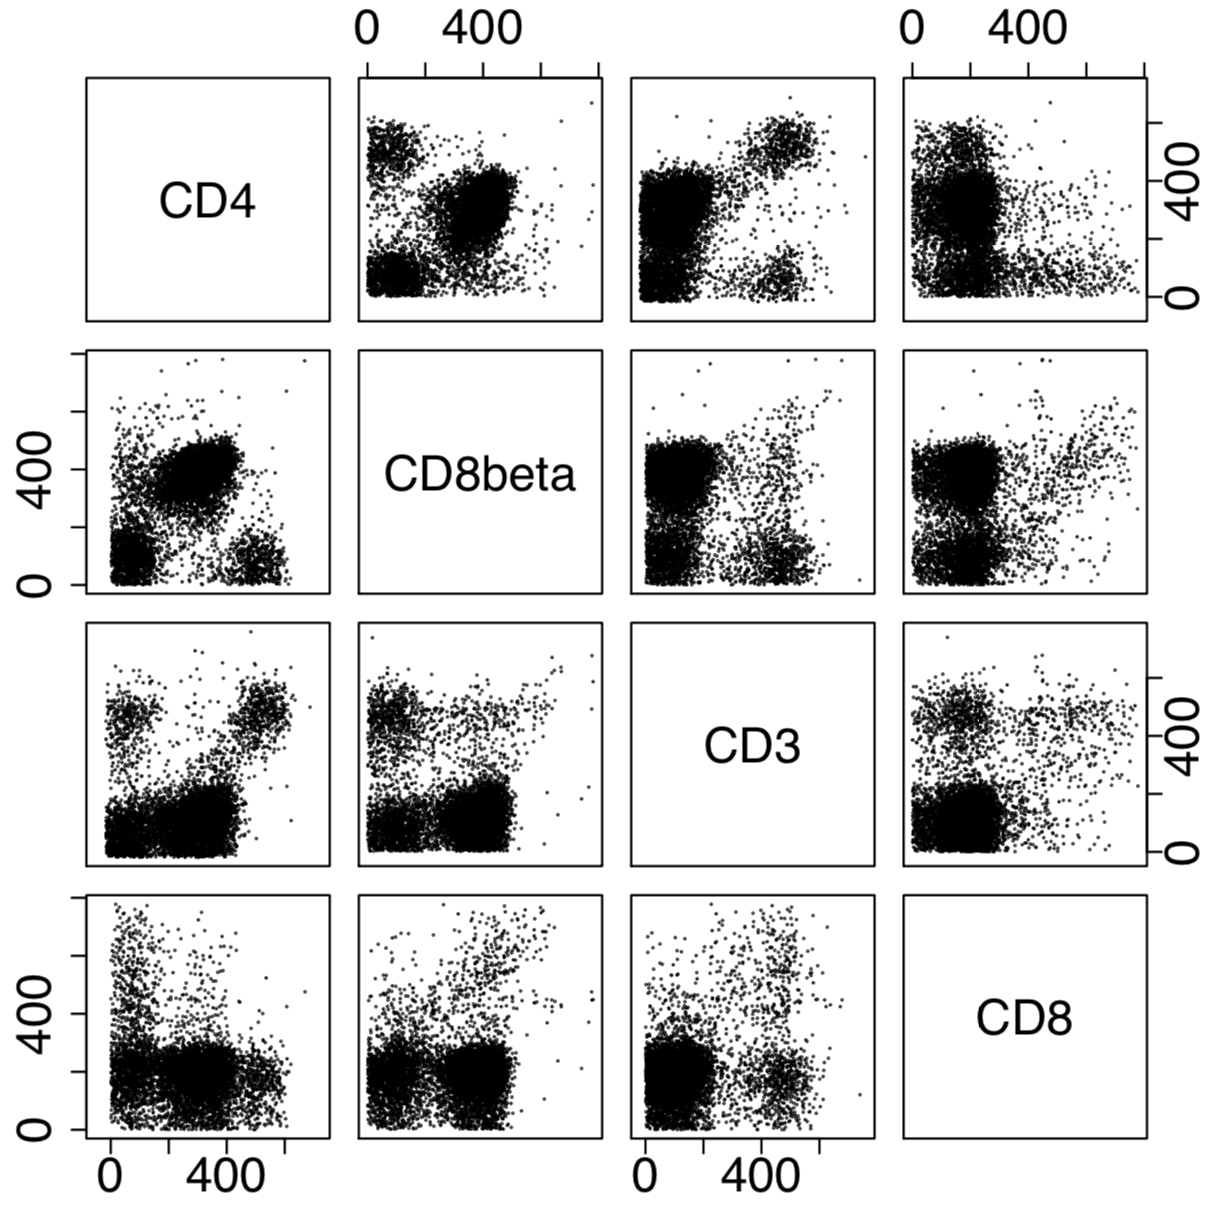
\includegraphics[width=0.7\linewidth]{scatter.png}
\end{center}
\end{frame}

\begin{frame}\frametitle{Strategy}
\begin{itemize}
\item
\alert{Cluster cells into cell populations} based on their 4 molecule levels
\bigskip
\item
Use \alert{threshold} to classify each group has having ``high'' or ``low'' levels of each molecule
\bigskip
\item
Plot concentrations of CD4 vs CD8$\beta$, \& \alert{only display groups with high levels of CD3} on plot
\begin{itemize}
\bigskip
\item
Allows us to identify cell populations with high levels of CD3, CD4, \& CD8$\beta$
\end{itemize}
\end{itemize}
\end{frame}

\begin{frame}\frametitle{Results for control individual (without disease)}
\begin{itemize}
\medskip
\item[]
\alert{NOTE}: Only clusters with high CD3 levels are shown
\end{itemize}
\begin{center}
\begin{minipage}{0.4\linewidth}
\includegraphics[width=\linewidth]{../Olson/Figures/d52_raw_2/merged_13_CD3_CD8beta.pdf}
\begin{center}
BIC solution
\\
$K = 13$
\\
Entropy $ = 3733$
\end{center}
\end{minipage}
\hfill
\begin{minipage}{0.4\linewidth}
\includegraphics[width=\linewidth]{../Olson/Figures/d52_raw_2/merged_10_CD3_CD8beta.pdf}
\begin{center}
Merged solution
\\
$K = 10$
\\
Entropy $= 58$
\end{center}
\end{minipage}
\end{center}
\end{frame}

\section{Conclusion}
\begin{frame}\frametitle{Summary}
\begin{itemize}
\item[]
BIC estimates \# of components well 
\bigskip
\item[]
ICL uses entropy to identify \# of groups well
\bigskip
\item[]
Baudry et al. combine their strengths:
\begin{itemize}
\bigskip
\item
Start with components from $\estim K_\text{BIC}$
\bigskip
\item
Use entropy to iteratively merge components
\end{itemize}
\end{itemize}
\end{frame}

\begin{frame}\frametitle{Discussion}
\begin{itemize}
\item[]
\alert{Key idea:} Allow submixtures as components, so that $\left(\# \text{ mixture components}\right)$ 
$\ne$ 
$\left(\# \text{ clusters} \right)$
\bigskip
\item[]
Honest density representations, much lower entropy
\bigskip
\item[]
Departs from model-based clustering, losing some of the appeal
\bigskip
\begin{itemize}
\item
Cannot choose $K$ as cleanly
\end{itemize}
\end{itemize}
\end{frame}

\begin{frame}\frametitle{References}
(1)
Biernacki, C., Celeux, G., and Govaert, G. (2000), ``Assessing a Mixture Model for Clustering With the Integrated
Completed Likelihood,'' IEEE Transactions on Pattern Analysis and Machine Intelligence, 22, 719-725.
\\ \bigskip
(2) Brinkman, R. R. et al. (2007), ``High-Content Flow Cytometry and Temporal Data Analysis for Defining a Cellular Signature of
Graft-versus-Host Disease,'' Biology of Blood and Marrow Transplantation, 13, 691-700.
\\ \bigskip
(3) Dasgupta, A., and Raftery, A. E. (1998), ``Detecting Features in Spatial Point Processes With Clutter via ModelBased
Clustering,'' Journal of the American Statistical Association, 93, 294-302. 
\end{frame}

\begin{frame}
\begin{center}
\Large
Questions?
\end{center}
\end{frame}

\begin{frame}\frametitle{Estimating $\estim z_{ik}$}
\begin{itemize}
\item[]
Conditional probabilities:
\ba
t_{ik}(\estim\theta_K) & = \Pr{\bx_i \text{ arises from component $k$} \mid \estim\theta_K } \\
	& = \frac{ p_k \phi_k(\bx_i | \mu_k, \Sigma_k)  }
 	{ \sum_{j=1}^K p_j \phi_j(\bx_i | \mu_j, \Sigma_j) }
\ea
with $\phi_k = $ $k$th Gaussian mixture density
\medskip
\item[]
MAP estimates:
\ba
\estim z_{ik} := \ind{ \argmax_{1 \le j \le K} t_{ij}(\estim\theta_K) = k }
\ea
\end{itemize}
\end{frame}

\begin{frame}\frametitle{Description of flow cytometry and manual gating}
\begin{itemize}
\item
Flow cytometry:
A biophysical technology employed in cell counting, cell sorting, biomarker detection, etc.
\medskip
\item
Fluorescence-activated cell sorting (FACS): special type of flow cytometry. Provides a method for sorting a heterogeneous mixture of biological cells into 2 or more containers, one cell at a time, based upon the specific light scattering and fluorescent characteristics of each cell
\medskip
\item
Gating: a process or sorting cells according to physical and fluorescence characteristics
\end{itemize}
\end{frame}

\begin{frame}\frametitle{Illustration: Comparing the $K = 2$ solutions}
\begin{center}

\begin{minipage}{0.45\linewidth}
\includegraphics[width=\linewidth]{../Olson/Figures/unif/merged_2_contour.pdf}
\begin{center}
Merged solution for $K = 2$
\end{center}
\end{minipage}
\hfill
\begin{minipage}{0.45\linewidth}
\includegraphics[width=\linewidth]{../Olson/Figures/unif/ICL2_contour.pdf}
\begin{center}
ICL solution ($K = 2$)
\end{center}
\end{minipage}
\end{center}
\end{frame}

\begin{frame}\frametitle{Full results for individual with disease}
\alert{NOTE}: Only CD3-positive clusters are shown
\begin{center}
\begin{minipage}{0.3\linewidth}
\includegraphics[width=\linewidth]{../Olson/Figures/d51_raw/ICL7_CD3_CD8beta.pdf}
\begin{center}
ICL solution
\\$K = 9$
\\Ent $=3235$ 
\end{center}
\end{minipage}
\hfill
\begin{minipage}{0.3\linewidth}
\includegraphics[width=\linewidth]{../Olson/Figures/d51_raw/merged_15_CD3_CD8beta.pdf}
\begin{center}
BIC solution
\\
$K = 13$
\\
Ent = 6251
\end{center}
\end{minipage}
\hfill
\begin{minipage}{0.3\linewidth}
\includegraphics[width=\linewidth]{../Olson/Figures/d51_raw/merged_12_CD3_CD8beta.pdf}
\begin{center}
Merged solution
\\
$K = 9$
\\
Ent = 1478
\end{center}
\end{minipage}
\end{center}
\end{frame}

\begin{frame}\frametitle{Full results for individual without disease}
\alert{NOTE}: Only CD3-positive clusters are shown
\begin{center}
\begin{minipage}{0.3\linewidth}
\includegraphics[width=\linewidth]{../Olson/Figures/d52/ICL4_CD3_CD8beta.pdf}
\begin{center}
ICL solution
\\
$K = 312$
\\
Ent $= 1901$
\end{center}
\end{minipage}
\hfill
\begin{minipage}{0.3\linewidth}
\includegraphics[width=\linewidth]{../Olson/Figures/d52/merged_13_CD3_CD8beta.pdf}
\begin{center}
BIC solution
\\
$K = 4330$
\\
Ent = 3733
\end{center}
\end{minipage}
\hfill
\begin{minipage}{0.3\linewidth}
\includegraphics[width=\linewidth]{../Olson/Figures/d52/merged_4_CD3_CD8beta.pdf}
\begin{center}
Merged solution
\\
$K = 4$
\\
Ent = 144
\end{center}
\end{minipage}
\end{center}
\end{frame}

\begin{frame}\frametitle{Example control data from Brinkman}

\begin{center}
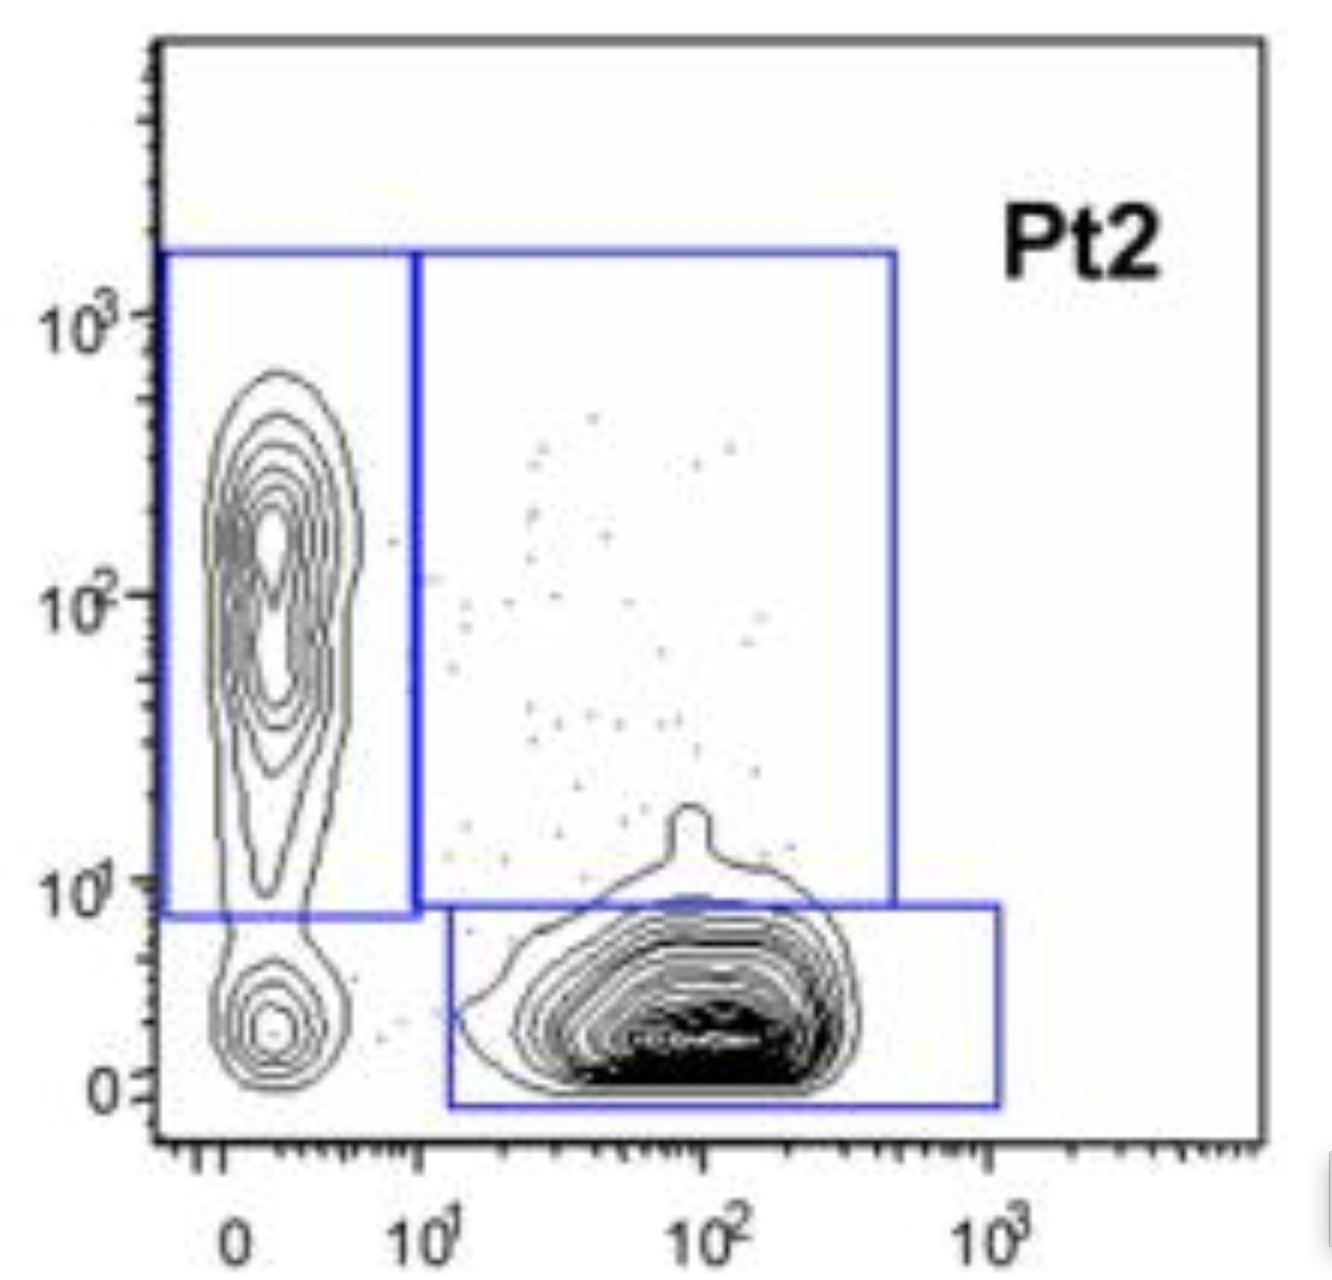
\includegraphics[width=0.7\linewidth]{Brinkman.png}
\end{center}
\end{frame}

\end{document}























